%!TEX root = ../thesis.tex

%% ----------------------------------------------------------------------------
% BIWI SA/MA thesis template
%
% Created 09/29/2006 by Andreas Ess
% Extended 13/02/2009 by Jan Lesniak - jlesniak@vision.ee.ethz.ch
%% ----------------------------------------------------------------------------
\newpage
\chapter{Materials}
% The objectives of the ``Materials'' section are the following:
% \begin{itemize}
%  \item \textit{What are tools and methods you used?} Introduce the environment, in which your work has taken place - this can be a software package, a device or a system description. Make sure sufficiently detailed descriptions of the algorithms and concepts (e.g. math) you used shall be placed here.
%  \item \textit{What is your work?} Describe (perhaps in a separate chapter) the key component of your work, e.g. an algorithm or software framework you have developed.
% \end{itemize}

\section{Workstation}

The main developing tool has been a laptop which has been used for a huge variaty of tasks: write code, debug, check papers and documentation, write notes, etc.
In order to train and make prediciton with deep learning models, an intensive computational resources are required.

This is why in addition, access to a GPU cluster has been provided in order to train models using GPUs.
The Computer Vision Lab provide access to BIWI cluster which has been used to store datasets and models and also as a computation resource. The BIWI cluster consists on 70 computational nodes (CPU only) with a total of 556 processors, 8328 cores and 13.3TB of RAM memory.
In addition, there are the GPU nodes which consists in 75 GPUs with 12GB of GPU memory each one.

\section{Software}

All the code developement has been done using the Python3 language.
Python is commonly extended in computer vision and deep learning applications because all the available libraries that provides computational frameworks and also because its easiness developing.

The main library used to develop deep learning models has been PyTorch~\cite{paszke2017automatic}. This library provides high-level features for tensor computation and deep neural networks.
This library is a wrapper in Python which under the hood is writen in C allowing fast performance and strong GPU acceleration.
This library is usually used in the research community because it

\section{Datasets}

During the development of this thesis, two segmentation datasets have been used: DAVIS and PASCAL.


\subsection{DAVIS Dataset}

The DAVIS Dataset \cite{Perazzi2016} consists on a Densely Annotated Video Segmentation dataset.
It provides a curated densely annotations for object instances in video sequences.
There are two versions of the dataset: 2016 and 2017. The 2016 version provides foreground/background annotations while the 2017 provides annotations for multiple objects and instances in the foreground.
During the work done on this thesis, DAVIS 2016 version has been used.
Some examples of the annotations are shown in Figure~\ref{fig:davis} and information about the dataset is also given in Table~\ref{table:davis}.

\begin{table}[h]
\centering
\begin{tabular}{l|lll}
DAVIS 2016                         & train & val  & \textbf{Total} \\
\hline
Number of sequences                & 30    & 20   & \textbf{50}    \\
Number of frames                   & 2079  & 1376 & \textbf{3455}  \\
Mean number of frames per sequence & 69.3  & 68.8 & \textbf{69.1}  \\
Number of objects per sequence     & 1     & 1    & \textbf{1}     \\
\end{tabular}
\caption{Size of the DAVIS 2016 data splits: number of sequences, frames and annotated objects.}
\label{table:davis}
\end{table}

\begin{figure}
\centering
\begin{subfigure}{0.25\textwidth}
  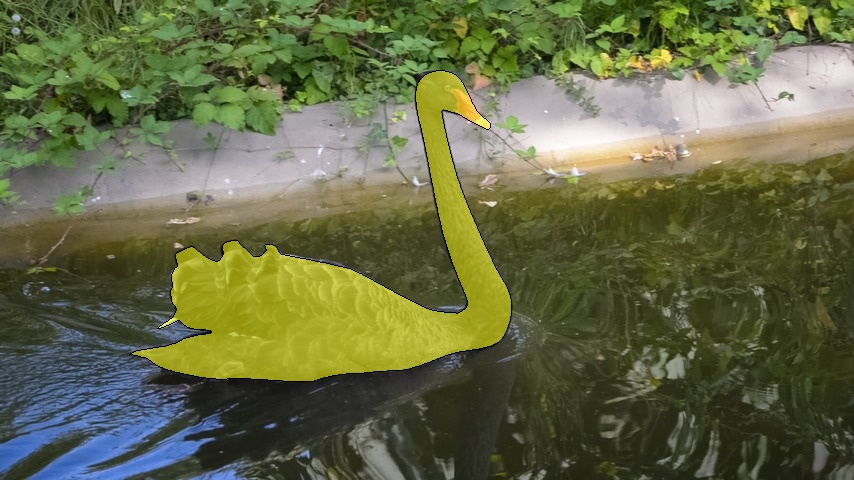
\includegraphics[width=1.\linewidth]{figures/davis_dataset/blackswan.jpg}
\end{subfigure}%
\begin{subfigure}{0.25\textwidth}
  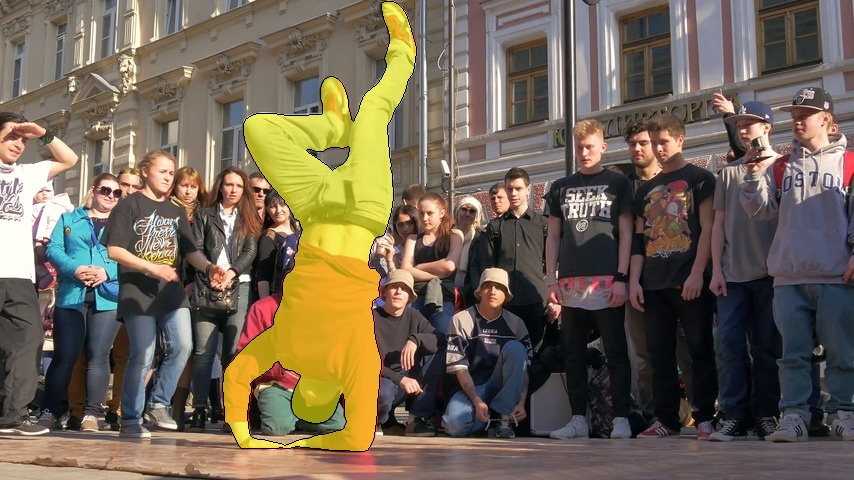
\includegraphics[width=1.\linewidth]{figures/davis_dataset/breakdance.jpg}
\end{subfigure}%
\begin{subfigure}{0.25\textwidth}
  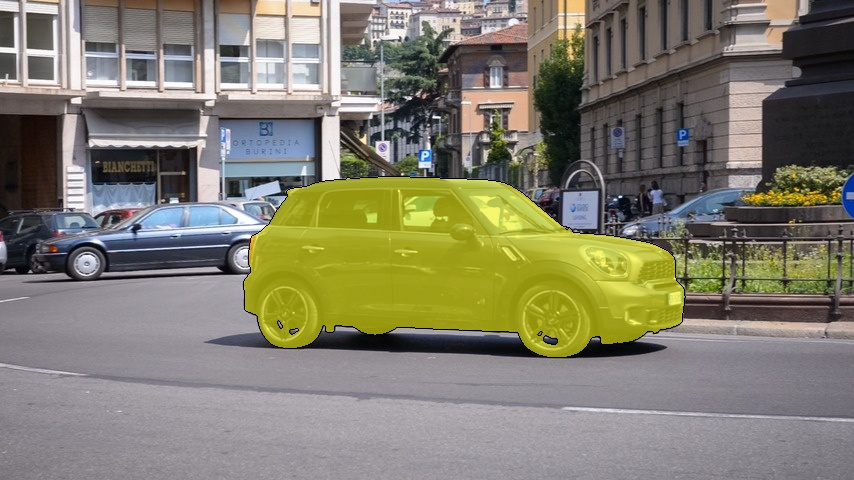
\includegraphics[width=1.\linewidth]{figures/davis_dataset/car-roundabout.jpg}
\end{subfigure}%
\begin{subfigure}{0.25\textwidth}
  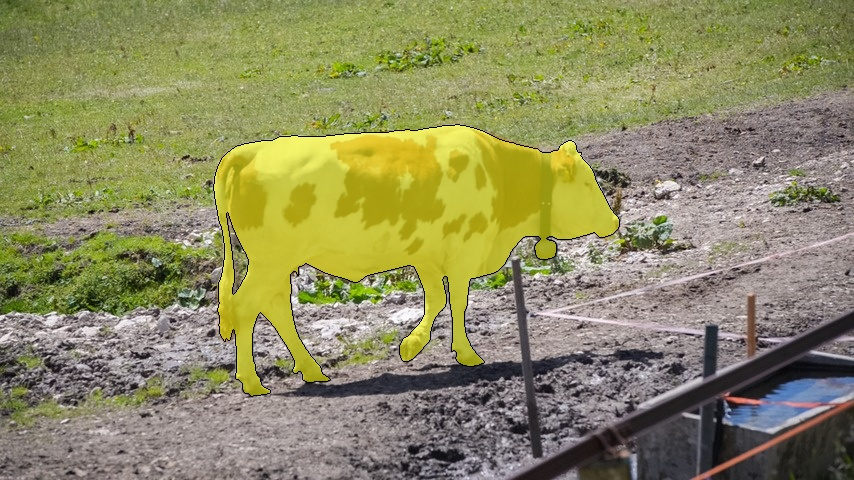
\includegraphics[width=1.\linewidth]{figures/davis_dataset/cow.jpg}
\end{subfigure}
\caption{Example of annotations on DAVIS Dataset.}
\label{fig:davis}
\end{figure}


The DAVIS dataset owners also organize a challenge to evaluate the performance of different segmentation method.
This challenge have two branches which are the following:

\paragraph{Semi-supervised}

Consists on generate a prediction given only the ground truth mask of the first frame.
This gives information to the about which is the object intended to be segmented.

\paragraph{Unsupervised}

As the name specifies, no information is given about the object that must be segmented.
To solve this, the segmentation methods rely on the frames to infer the foreground and background.

\subsection{PASCAL Dataset}

PASCAL Dataset~\cite{Everingham10} is a dataset used to benchmark vision object category recognition, detections and segmentation.
Consist on images containing 20 visual object classes and provides multiple annotation for different computer vision tasks: detection and segmentation.
The segmentation annotations consist on masks over instances belonging to the 20 classes, which lead with images with multiple instance annotations.

During this thesis, the segmentation annotations from PASCAL VOC 2012 have been used. The information about the number of instances per split can be found on Table~\ref{table:pascal}.

\begin{table}[h]
\centering
\begin{tabular}{l|lll}
PASCAL VOC 2012                    & train & val  & \textbf{Total} \\
\hline
Number of images                & 1464    & 1449   & \textbf{2913}    \\
Number of instances           & 3507 & 3427 & \textbf{6934} \\
Mean number of instances per image & 2.40  & 2.37 & \textbf{2.38}  \\
\end{tabular}
\caption{Size of the PASCAL VOC 2012 data splits: number of images and annotated objects.}
\label{table:pascal}
\end{table}
